
\section{Learning about motion}


The robot tracks how an object moves after impact.
Pooling this data over all objects reveals how the movement of
the robot's arm correlates with the final movement of the object.

The robot was sensitive to color histogram, principal axis.
%
Some objects have preferred directions of motion.  For example,
a toy car tended to roll forward along its principal axis.
%
[Need a lot more here].
%
%%Figures~\ref{fig:observed-action} and \ref{fig:mimicked-action}.
Figure \ref{fig:mimicked-action}.


\ifnote
\begin{figure}[tb]
\begin{center}
%%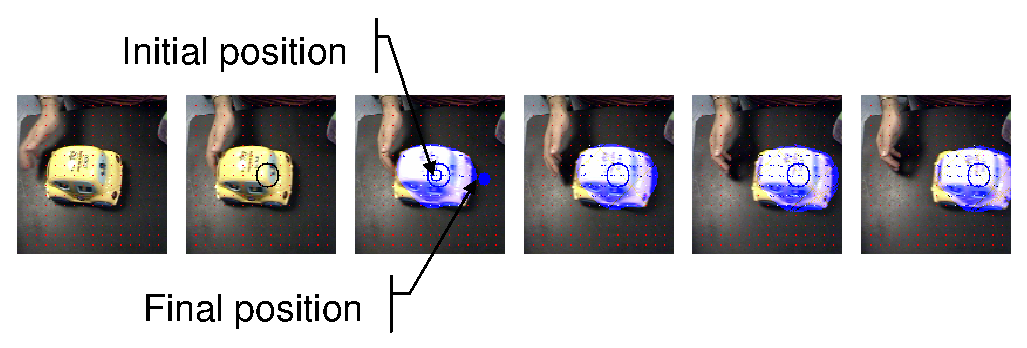
\includegraphics[width=\columnwidth]{observed-action.eps}
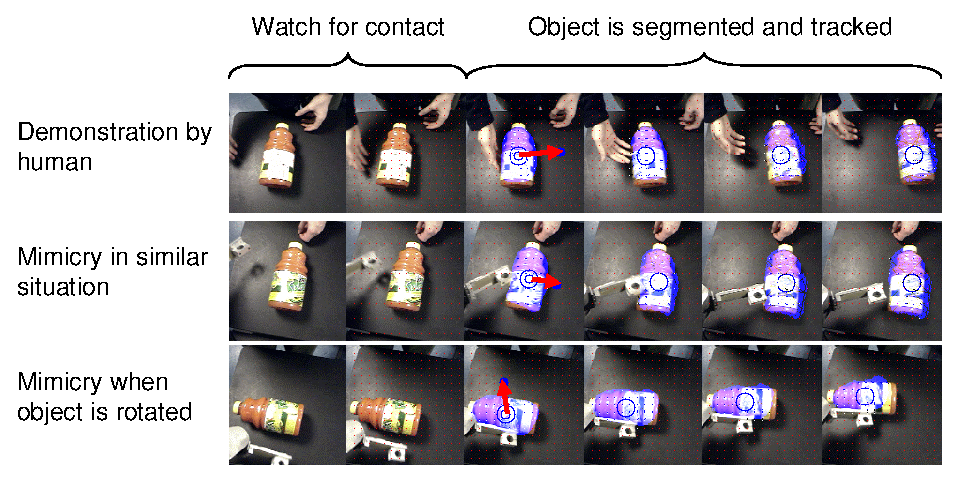
\includegraphics[width=\columnwidth]{fig-mimicry-bottle}
\caption{ 
\label{fig:observed-action}
%
Basic mimicry.  The first step in mimicking an action is to actually
be able to observe it.  The first sequence shows a human demonstration
of a poking operation.  Frames around the moment of contact are shown.
The object, after segmentation, is tracked for 12 frames using a
combination of template matching and optic flow.  The big circles
represent the tracked position of the bottle in successive frames.
The arrow displayed on the frame of contact ($3^{rd}$ from the left)
projects from the position at the time of contact and at the $12^{th}$
frame respectively.
%
In the second sequence, the bottle is presented to the robot in the
same orientation it had in the demonstrated action and the robot
repeats the observed action, a ``side tap''.  In the third sequence,
the car is presented at a different angle.  The appropriate action to
exploit the affordance and make the bottle roll is now a ``back
slap''.
%
%An example of observed sequence with tracking superimposed. 
%Frames around the
%moment of contact are shown. The object, after segmentation, is tracked for 12 
%frames using a combination of template matching and optic flow. The big circles
%represent the position of the toy car in successive frames. The two small circles
%(outline and solid) displayed on the frame of contact ($3^{rd}$ from the left) are 
%the position at the time of contact and at the $12^{th}$ frame respectively.
%
}
\end{center}
\end{figure}
\fi

\begin{figure}[tb]
\begin{center}
%%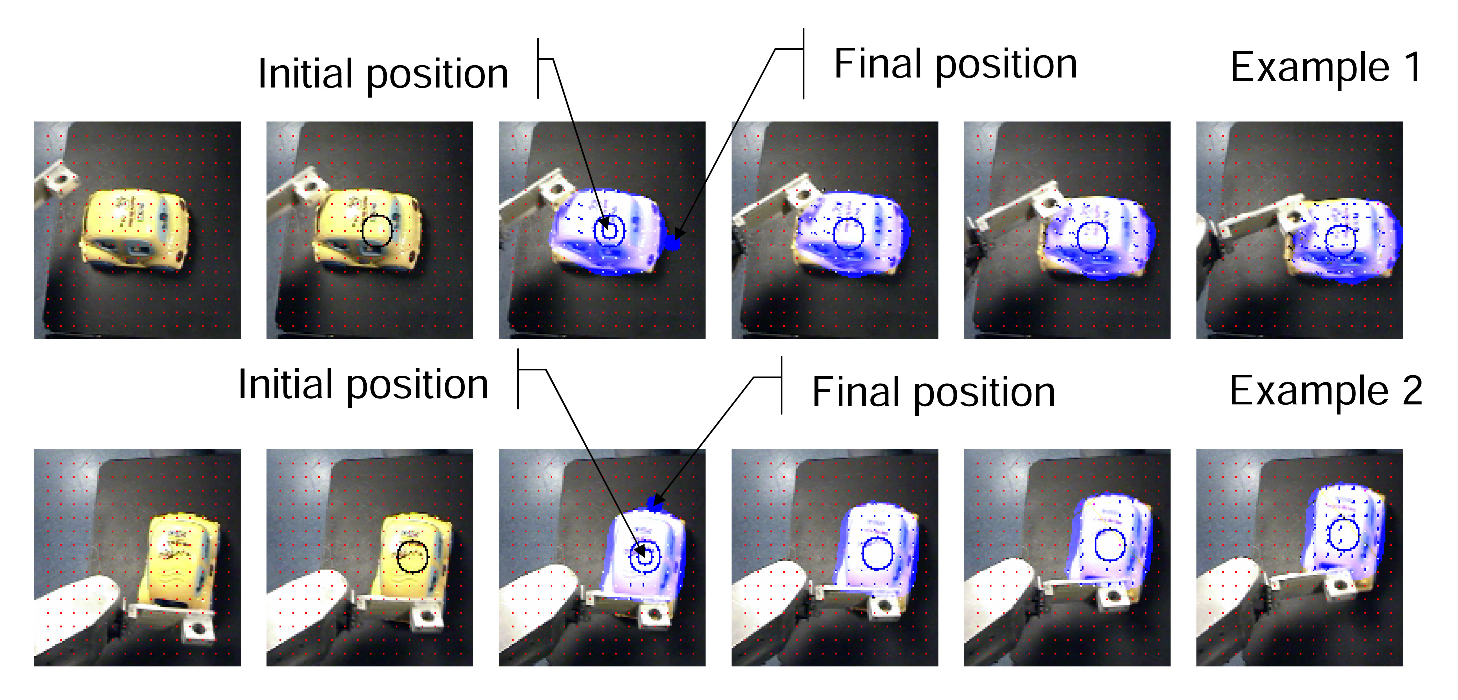
\includegraphics[width=\columnwidth]{mimicked-action.eps}
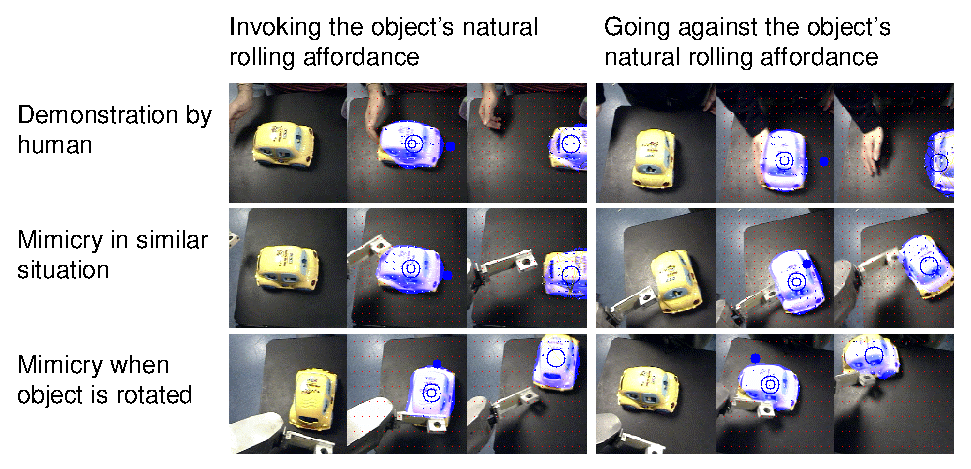
\includegraphics[width=\columnwidth]{fig-mimicry-awkward.eps}
\caption{ 
\label{fig:mimicked-action}
%
An extended mimicry example using the toy car.
The sequences on the left show the robot mimicking a human exploiting
the car's rolling affordance.  The sequences on the right show
what happens when the human hits the car in a contrary fashion, going
against its preferred direction of motion.  The robot mimics this 
``unnatural'' action, suppressing its usual behavior of trying to
evoke rolling.
%OUTDATED Two examples of mimicry following the observation in figure \ref{fig:observed-action} 
%where a human manipulator pokes the toy car exploiting the affordance (the car rolls). 
%In example 1 (top row), the toy car has the same orientation it had in the
%demonstrated action and the robot repeats the observed action. In example 2 (bottom), 
%the car is $90^\circ$ with respect to example 1. The appropriate action to exploit
%the affordance and make the car roll is thus a back slap. 
%
}
\end{center}
\end{figure}

